\label{cha:grundlagen}
Als Fundament für die weitere Arbeit sollen zunächst eine Grundlagen erarbeitet werden. Um das Vorhaben und die Schritte dieser Arbeit besser nachvollziehen zu können, wird zunächst das Modell der \textit{Tetrade der Medieneffekte} vorgestellt. \textbf{Hierbei handelt es sich um eine Idee von Marshall McLuhan, welcher sich mit den Effekten beschäftigt, die ein Medium mit sich bringt. Er hat festgestellt, dass es im Wesentlichen vier Effekte von Interesse sind, welche er mit den folgenden Fragen bestimmen will \citep{mcluhan1977laws}}:

\begin{enumerate}
\item What does the medium enhance?
\item What does the medium make obsolete?
\item What does the medium retrieve that had been obsolesced earlier?
\item What does the medium reverse or flip into when pushed to extremes?
\end{enumerate}

So stellt \cite{mcluhan1977laws} fest, dass \textbf{das} Radio eine unmittelbare und auditive Art der Kommunikation beförderte. Im gleichen Moment wurden dadurch die Bedeutsamkeit von Printmedien geschwächt. Hierdurch hat die vorangegangene auditive Kommunikation, welche durch die Einführung von Printmedien obsolet wurde, wieder an Bedeutung gewonnen. Wenn man nun das Medium an sein Limit bringt, dann befördert dies die Entwicklung hin zum Fernsehen \citep{mcluhan1977laws}.

Mit diesen Gedanken im Hinterkopf werden nun die Grundlagen für diese Arbeit betrachtet. Alle in den Grundlagen betrachteten Themen beschäftigen sich ebenfalls mit Medien und deren Effekten. \textbf{Zuletzt} soll auch in Kapitel \ref{cap:evaluation} der Kreis geschlossen werden und das Medium Hyperaudio-Dokument nochmals anhand der \textit{Tetrade der Medieneffekte} bewertet werden.


\section{Moodle}
\label{sec:moodle}
Bei Moodle (Modular Object-Oriented Dynamic Learning Environment) handelt es sich im Wesentlichen um ein frei verfügbares Open Source Learningmanagementsystem (GNU Public License), mit dem Internet-basierte Kurse entwickelt und durchgeführt werden können \citep{moodle2015was}. Ziel der Lernplattform ist es, den Lehrenden, Administratoren und Lernenden ein robustes, sicheres und integriertes System zu liefern, mit dessen Hilfe sie eine personalisierte Lernumgebung gestalten können \citep{moodle2018about}. Unter dieser Zielsetzung \textbf{ist Moodle weltweit als Lernplattform weit verbreitet} und hat aktuell 101.447 registrierte Seiten in 232 Ländern mit insgesamt mehr als 130 Millionen Benutzern \citep{moodle2018stats}. Im Folgenden wird der Aufbau einer Moodle-Seite geschildert.

Zugriff auf Moodle erhält der Nutzer über die Startseite, welche auf die eigenen Bedürfnisse angepasst werden kann. Auch kann Moodle so konfiguriert werden, dass die Startseite erst nach Anmeldung an der Login-Seite erfolgen kann. Die Grundstruktur von Moodle ist, wie in Abbildung \ref{fig:MoodleAufbau} zu sehen, anhand von Kursbereichen und Kursen organisiert. Kurse werden wiederum als Seiten repräsentiert, auf welchen die Lehrenden Arbeitsmaterialien und Aktivitäten für die Studierenden bereitstellen können. Kurse werden üblicherweise in einzelne Kursabschnitte unterteilt, in welchen die Arbeitsmaterialien und Aktivitäten eingebunden werden. Kursseiten können mittels Blöcken noch um weitere zusätzliche Informationen angereichert werden.

Ein Beispiel für eine Kursseite ist in Abbildung \ref{fig:MoodleKursseitenbeispiel} anhand des Kurses \glqq Einführung in Mensch-Computer-Interaktion\grqq{} zu sehen. Auf der linken Seite sind innerhalb der Navigation die einzelnen Kursabschnitte, hier als Kurseinheiten beziehungsweise Einführung  benannt, sichtbar. Unterhalb der Navigation, sowie auf der rechten Seite sind die verschiedenen Blöcke (z.B. \glqq Aktivitäten\grqq{}, \glqq Suche in Foren\grqq{} oder \glqq Neue Ankündigungen\grqq{}) innerhalb des Kurses angeordnet. Im mittleren Bereich befinden sich untereinander die Beschreibungen der einzelnen Kursabschnitte, mit Links zu den verwendeten Arbeitsmaterialien und Aktivitäten.

Kurse werden dann innerhalb von Kursbereichen organisiert. Hierbei ist auch ein mehrstufiges Kursbereichssystem umsetzbar \citep{moodle2015aufbau}.

\begin{figure}[h!]
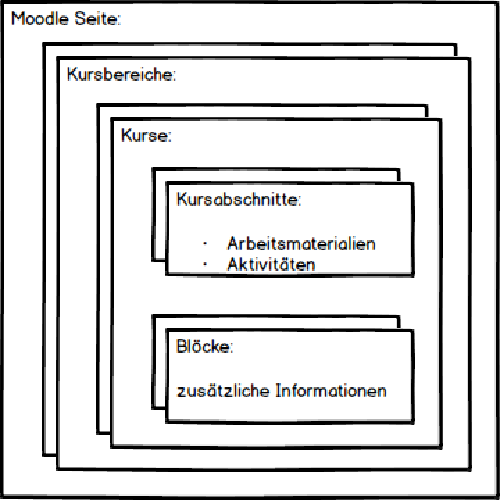
\includegraphics[width=.5\textwidth,center]{MoodleAufbau.pdf}
\caption{\label{fig:MoodleAufbau}Schematischer Aufbau einer Moodle Seite}
\end{figure}

\begin{figure}[h!]
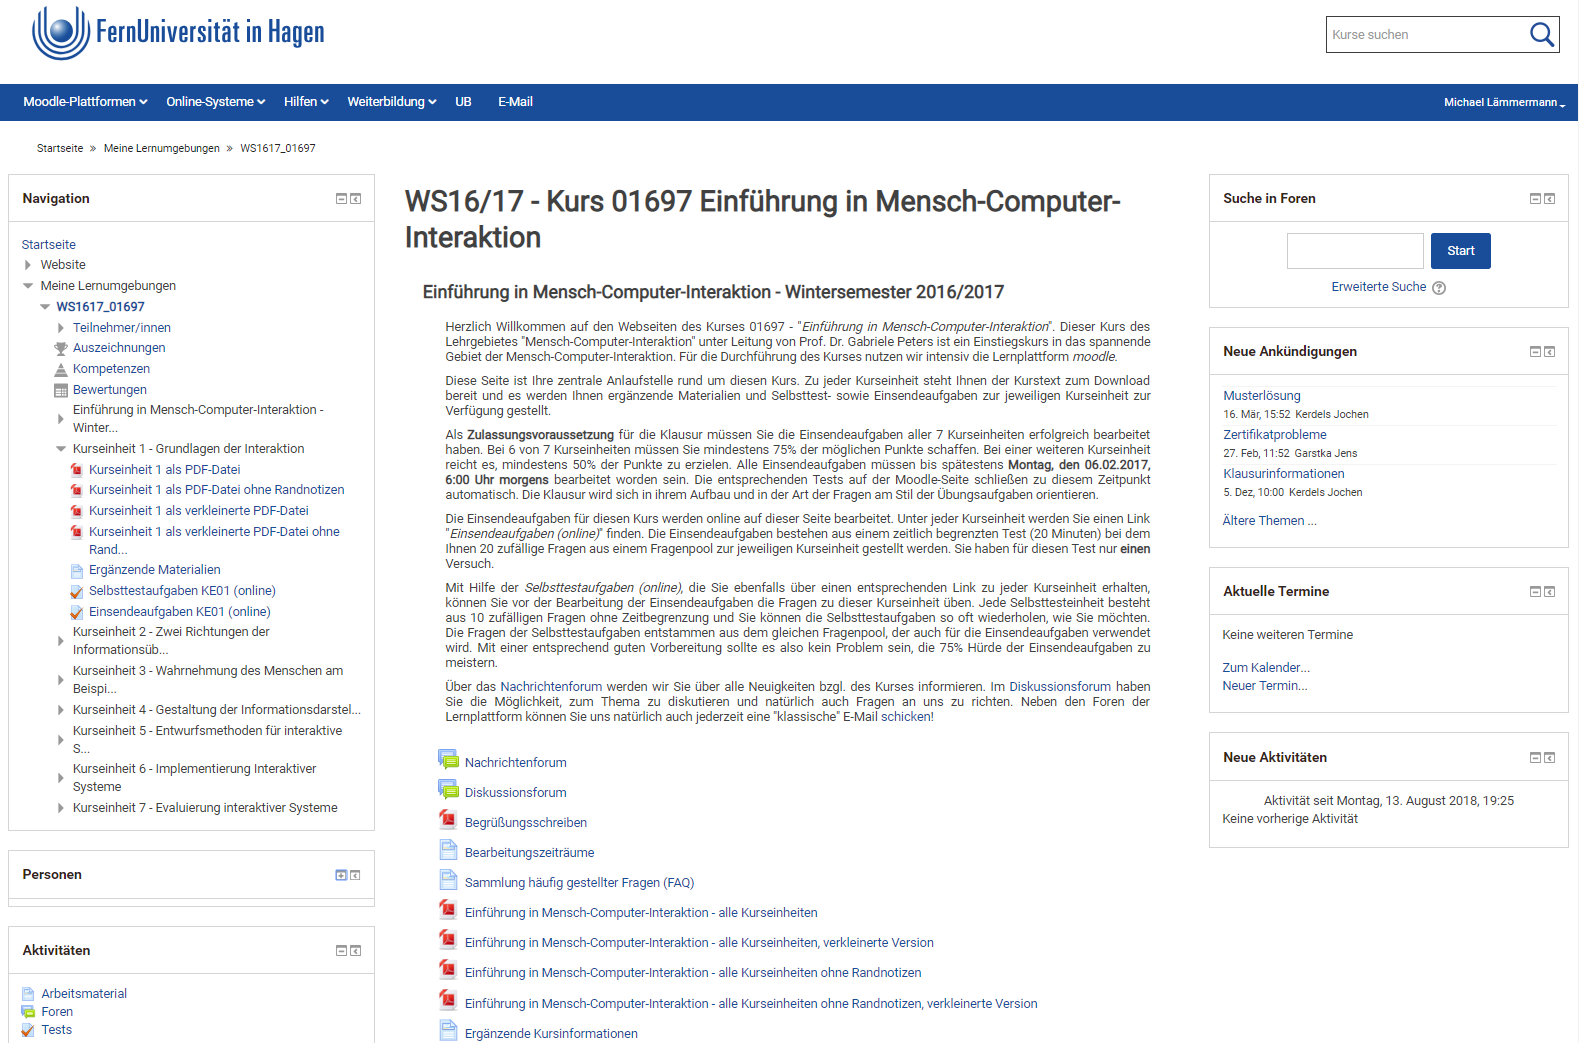
\includegraphics[width=\textwidth,center]{MoodleKursseitenbeispiel.png}
\caption{\label{fig:MoodleKursseitenbeispiel}Kursseite des Kurses \glqq Einführung in Mensch-Computer-Interaktion\grqq{} \citep{fernuniversitaet2018mensch}}
\end{figure}

%behauptung?
Technisch baut Moodle auf dem für eine Webanwendung üblichen Aufbau aus Webserver und Datenbank unter Verwendung von PHP auf. Um die zum Ziel gesetzte Personalisierbarkeit zu erreichen, setzt Moodle unter anderem auf ein Plugin-System. \textbf{Plugins werden in über 50 verschiedene Plugin-Typen kategorisiert, wobei jeder dieser Typen dazu dient, einen speziellen Bereich von Moodle zu erweitern beziehungsweise anzupassen \citep{moodle2017plugin}}.


%%%%%%%%%%
\section{Kooperation im Lernumfeld}
\glqq Lernen ist in vieler Hinsicht ein sozialer Prozess, der kulturelle Einflüsse einschließt sowie soziale Aktivitäten und gemeinsames Problemlösen umfasst\grqq{} \citep{reinmann1995kooperation}. %Diese Aussage macht die Bedeutung von Kooperation im Lernumfeld klar. 
\todo[inline]{Verknüpfung}
\textbf{Während in dieser Arbeit, wie im deutschsprachigen Raum üblich, keine Unterscheidung zwischen dem \textit{kooperativen} und dem \textit{kollaborativen} Lernen vorgenommen wird, werden die Begriffe außerhalb des deutschsprachigen Raums häufig differenziert betrachtet \citep{reinmann2002analyse}. Eine differenzierte Betrachtung der beiden Begriffe liefert \cite{dillenbourg1995evolution}. Demnach handelt es sich um \textit{Kooperation}, wenn eine Problemlösung durch die Arbeitsteilung unter den Mitgliedern einer Gruppe erreicht wird, wobei jedes Mitglied für einen Teil der Problemlösung verantwortlich ist.
%cooperation "... is accomplished by the division of labor among participants, as an activity where each person is responsible for a portion of the problem solving..."
Bei \textit{Kollaboration} wird die Problemlösung hingegen durch gemeinsames Engagement der Gruppenmitglieder bei koordiniertem Vorgehen zur Problemlösung erreicht.} %\citep{dillenbourg1995evolution}}.
%collaboration "... mutual engagement of participants in a coordinated effort to solve the problem together"
\todo[inline]{Beispiele}
%Im Folgenden wird, wie für den deutschsprachigen Raum üblich, keine Unterscheidung zwischen dem kooperativen und dem kollaborativen Lernen vorgenommen \citep{reinmann2002analyse}. 
Weitgefasst versteht man unter kooperativem Lernen eine Situation, in der zwei oder mehrere Personen zusammen lernen oder versuchen, zusammen zu lernen \citep{dillenbourg1999collaborative}. Da Kooperation auch einen zentralen Aspekt des zu entwickelnden Moodle-Plugins darstellt, wird nochmals auf die Kooperation beim Lernen sowohl in offline- als auch in online-Lernumgebungen betrachtet.

%Variety of Scale
%Variety of Meaning for Learning
%Variety of Meaning for Learning

%Was will ich hier überhaupt erzählen?


%Can a Hypermedia Cooperative e-Learning Environment Stimulate Constructive Collaboration?
%The efficacy of online cooperative learning systems
%Warum Kooperation neu erfinden? Zum Beitrag der CSCW-Forschung für das kollaborative E-Learning 

%%%%%%%%%%
\subsection{Offline}
%https://de.wikipedia.org/wiki/Kooperatives_Lernen#cite_note-1
\citep{reinmann1995kooperation}
\citep{reinmann2002analyse}
\citep{pauli2000rolle}

%%%%%%%%%%
\subsection{Online}

\citep{dillenbourg1999collaborative}


%%%%%%%%%%
\section{Hypermedia}
\textbf{Bevor mit der genauen Konzeption und Implementation des Moodle-Plugins für Hyperaudio-Dokumente begonnen werden kann, werden zunächst \textit{Hypermedia} im Allgemeinen betrachtet}. Dabei soll zunächst eine Begriffsklärung durchgeführt werden. Darauf aufbauend werden einige Erfahrungen aus verschiedenen wissenschaftlichen Arbeiten gesammelt. \textbf{Zuletzt können daraus Rückschlüsse für das zu entwickelnde Moodle-Plugin und die zugrundeliegende Interpretation von Hyperaudio gezogen werden.}

%%%%%%%%%%
\subsection{Grundbegriffe}
Hyperaudio stellt eine Ausprägung von \textit{Hypermedia} dar. Der Begriff \textit{Hypermedia} wurde das erste Mal von Ted Nelson 1965 verwendet \citep{nelson1965complex}. In seinem Paper beschreibt er detailliert, was er sich unter einem \textit{Hypertext} vorstellt. Hierunter versteht er ein Dokument bestehend aus geschriebenen oder bildhaften Inhalten, welche in solch einer komplexen Art und Weise miteinander verbunden sind, dass sie nicht mehr auf Papier dargestellt werden können. Es kann Zusammenfassungen, Karten über die Inhalte und deren Zusammenhänge, Annotationen, Ergänzungen oder Anmerkungen von Wissenschaftlern, die das Dokument begutachtet haben, enthalten. Nelson beschreibt das Kriterium für den Präfix \textit{hyper} damit, dass diese Objekte nicht durch eine Konvertierung in ein einfaches lineares Medium, wie beispielsweise einen String umgewandelt werden können. Der wesentliche Punkt ist also, dass es sich beim Lernen mit \textit{Hypermedia} um ein nicht-lineares Lernen handelt.

Genauer betrachtet stellt das, was Nelson sich damals als \textit{Hypertext} vorgestellt hatte, nach heutiger Definition bereits eine Form von \textit{Hypermedia} dar. Auch wenn viele die beiden Begriffe \textit{Hypertext} und \textit{Hypermedia} synonym verwenden \citep{nielsen2013multimedia}, werden bei strikter Betrachtung bei \textit{Hypertext} ausschließlich Texte miteinander verbunden, während bei \textit{Hypermedia} auch andere Medien eingebunden werden können. Gemeinsam haben beide Arten jedoch, dass der Lernende keinen linearen Weg vorgegeben hat, sondern von einem Knoten (Node) zum anderen springen kann und sich somit seinen Lernweg selbst aussucht. Als Folge dessen stellt \textit{Hypermedia} eine nicht-lineare Variante von \textit{Multimedia} dar.

Nach dieser Logik handelt es sich bei Hyperaudio in seiner klassischen Form eigentlich um reine Audiosequenzen, die miteinander verknüpft sind, wobei der Lernende selbst entschieden kann, in welcher Reihenfolge er diese abspielt \citep{zumbach2006learning}.


%%%%%%%%%%
\subsection{Lernen mit Hypermedia}
Wissenschaftler beschäftigen sich schon seit vielen Jahren damit, festzustellen, welche Effekte der Einsatz von \textit{Multimedia}, \textit{Hypertext} und \textit{Hypermedia} auf den Lernerfolg von Lehrenden hat. In der Arbeit von \cite{moos2010multimedia} wird eine Analyse von etlichen Arbeiten zu diesem Thema durchgeführt. \cite{moos2010multimedia} konzentrieren sich hierbei vor allem auf den Einfluss auf die Motivation der Lernenden. Dennoch wird auch auf andere Aspekte der drei verschiedenen E-Learning Methoden \textit{Multimedia}, \textit{Hypertext} und  \textit{Hypermedia} im Vergleich zu klassischen Lehrmethoden eingegangen.

\cite{moos2010multimedia} verweisen auf Arbeiten, nach denen eine Herausforderung bei \textit{Multimedia} und somit auch bei \textit{Hypermedia} darin besteht, dass die kognitive Aufnahmekapazität der Studierenden überschritten werden kann (Mayer und Moreno; van Merrienboer und Ayres, nach \cite{moos2010multimedia}), wenn Informationen sowohl aus einem Text als auch aus einem Diagramm entnommen werden sollen. Dies beruht auf der Annahme der Cognitive Load Theory, welche dem Arbeitsgedächtnis nur eine begrenzte Kapazität zuspricht (Sweller; van Merrienboer und Sweller, nach \cite{moos2010multimedia}). Es gibt aber auch Studien, welche einen positiven Effekt nachweisen, wenn zur gleichen Zeit Bilder dargestellt werden und dazu passender Text vorgelesen wird, im Vergeleich zum alleinigen Betracheten von Bildern beziehungsweise Anhören von Texten (Mayer und Anderson; Mayer und Sims, nach \cite{moos2010multimedia}).

\textit{Hypertext} bietet zwar Vorteile, da der Studierende den Lernweg bestimmen kann, der am besten auf seine Bedürfnisse angepasst ist. Auf der anderen Seite ist hierzu aber eine ausreichende Vorkenntnis in dem Lernbereich notwendig, um die Entscheidung, wie dieser Weg aussehen soll, treffen zu können. Des Weiteren wirkt sich auch ein fehlendes Interesse des Studierenden negativ auf die Effektivität der \textit{Hypertext}-Lernumgebung aus (Lawless und Kulikowich, nach \cite{moos2010multimedia}).
\todo[inline]{Zitat nochmals prüfen}

Es ist nun also nicht verwunderlich, dass \textit{Hypermedia} als Verschmelzung von \textit{Multimedia} und \textit{Hypertext} ebenfalls einige Herausforderungen mit sich bringt \citep{moos2010multimedia}. Scott und Schwartz (nach \cite{moos2010multimedia}) fordern für das Lernen mit \textit{Hypermedia} eine Balance zwischen effektiver Navigation und Inhaltsverständnis. Dies soll durch Prozesse zur Überwachung des eigenen Lernfortschritts erreicht werden, doch Untersuchungen haben ergeben, dass viele Studierende Schwierigkeiten dabei haben, diese Prozesse korrekt anzuwenden \citep{moos2010multimedia}.

\todo[inline]{Buch von Mayer - Seite: 172ff }
\label{sec:audiocues}
\todo[inline]{Hyperaudio: Audio Cues - Donker}

\textbf{Nachdem nun die Begrifflichkeiten um \textit{Hypermedia}, sowie den Begriff Hyperaudio im eigentlichen Sinne beleuchtet und entsprechende Studien betrachtet wurden, wird nun darauf eingegangen, welche Rückschlüsse daraus für diese Arbeit gezogen werden können}.

Zum einen ist festzustellen, dass wir den Begriff Hyperaudio nicht im ursprünglichen Sinn verwenden. Bei den Hyperaudio-Dokumenten im Sinne dieser Arbeit handelt es sich eigentlich um Multimedia-Dokumente. Erst unter Berücksichtigung der Kommentarfunktion und der Galerie wird der Hypermedia-Aspekt erfüllt. Der Zuhörer hat also die Möglichkeit von Kommentar zu Kommentar oder von Annotation zu Annotation zu springen und gelangt dabei an die entsprechende Stelle in der Audiosequenz. In Ergänzung zu \cite{zumbach2006learning} wird in dieser Arbeit unter Hyperaudio eine Audio-Datei verstanden, die durch die Erweiterung mittels Annotationen und Kommentarfunktion um Multimedia- und Hypermedia-Elemente ergänzt wird.
\todo[inline]{Galerie?}

Der Vorteil \textbf{dieser} Betrachtungsweise von Hyperaudio liegt darin, dass die Herausforderungen, die in Verbindung mit \textit{Hypermedia} bzw. \textit{Hypertext} normalerweise auftreten, nicht besonders prägnant sind. Im zu entwickelnden Moodle-Plugin wird dem Studierenden in erster Linie eine lineare Audio-Datei vorgespielt, die um Multimedia-Elemente ergänzt wird. Erst durch den Einsatz der Galerie und der Kommentarfunktion kommen die herausfordernden Elemente von Hypermedia ins Spiel. \textbf{Dementsprechend stellt das Hyperaudio-Plugin einen guten Kompromiss zwischen den verschiedenen Lehrmethoden dar}.
\todo[inline]{Galerie?}


%%%%%%%%%%
\section{Hyperaudio-Dokument}
\label{sec:hyperaudio}
\todo[inline]{Herleitung des Hyperaudio-Dokuments -> Entwicklung von Kurseinheit zu Hyperaudio -> Rückschluss auf Tetrade der Medieneffekte}
\todo[inline]{Nur Hyperaudio, nicht -Dokument. Dieser Abschnitt sollte m.E. früher, jedenfalls vor dem Lernen mit Multimedia, behandelt werden. }


%%%%%%%%%%
\section{Zusammenfassung}
\dots